\chapter{Prezentacja wyników}

Przeprowadzone zostały testy dla zaimplementowanych metod komunikacji. Wszystkie miały charakter lokalny (transmisja sieciowa wykorzystywała \textit{localhost}). Sprawdzone zostały różne rozmiary żądań i odpowiedzi w wielu kombinacjach (16B - 128MiB). Generowanie danych opisane zostało w rozdziale \ref{data_generation}.

Wszystkie uruchomienia korzystały z tej samej platformy:
\begin{itemize}
    \item System operacyjny: Ubuntu 17.10
    \item Java 9.0.1+11
    \item Procesor: intel i5 4690k
    \item Pamięć RAM: 16GB 2400MHz CL10
    \item dysk SSD (odczyt 250 MB/s, zapis 500MB/s, 72000 IOPS)
\end{itemize}


\section{Rozkład danych}

Każda konfiguracja testowa wykonana została co najmniej 1000-krotnie. Z otrzymanych wyników obliczona została średnia arytmetyczna oraz odchylenie standardowe, ponieważ ich wykresy zbliżone są rozkładu normalnego. Poniżej znajdą się diagramy, które to ukazują (dla wybranych metod).


\begin{figure}[H]
    \centering
    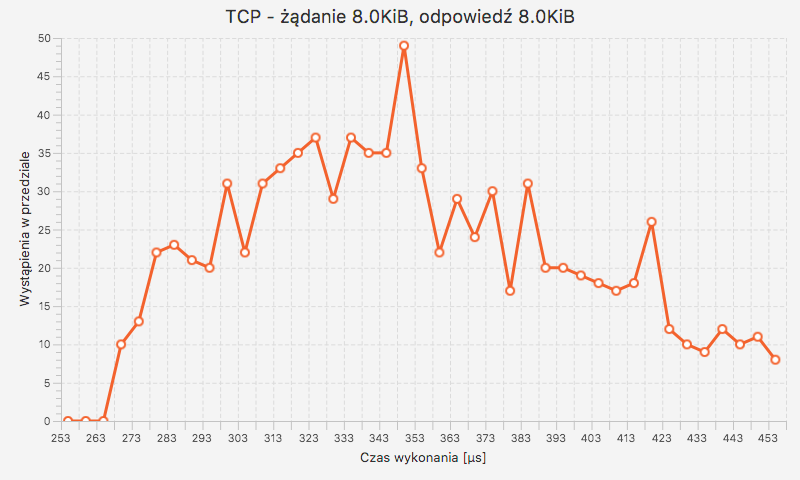
\includegraphics[scale=0.38]{img/charts/TCP_chart_8192_8192.png}
    \caption{Przykładowy wykres rozkładu czasów wykonania dla TCP}
\end{figure}

\begin{figure}[H]
    \centering
    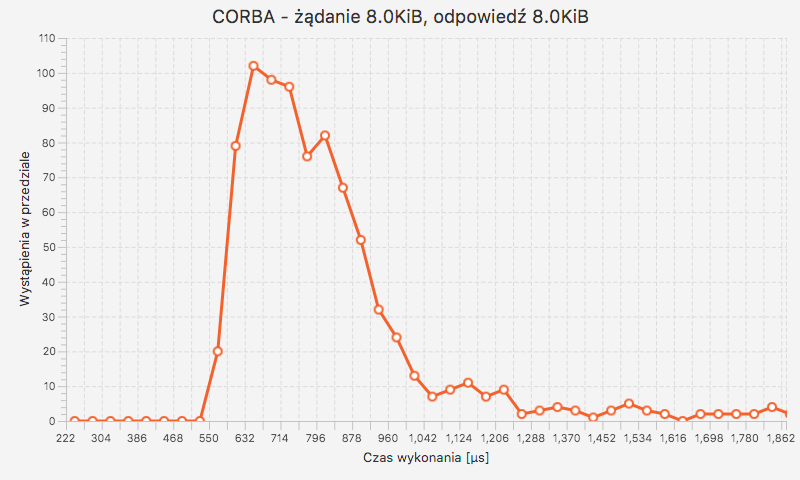
\includegraphics[scale=0.38]{img/charts/CORBA_chart_8192_8192.png}
    \caption{Przykładowy wykres rozkładu czasów wykonania dla technologii CORBA}
\end{figure}

\begin{figure}[H]
    \centering
    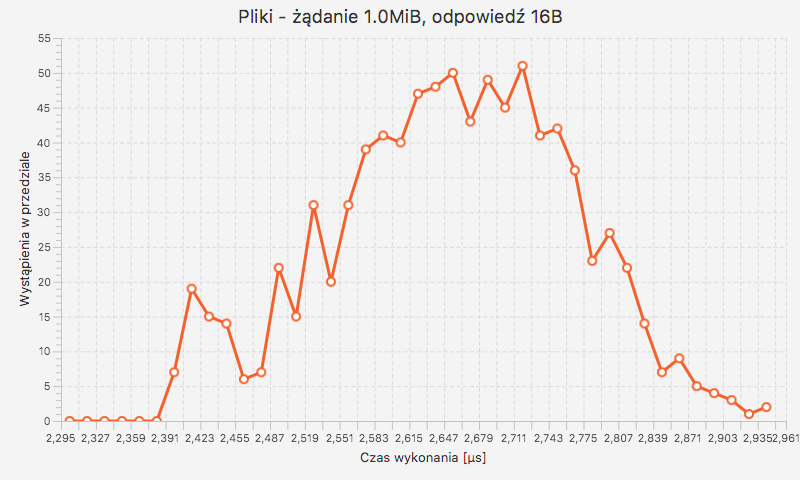
\includegraphics[scale=0.38]{img/charts/FILE_chart_1048576_16.png}
    \caption{Przykładowy wykres rozkładu czasów wykonania dla plików}
\end{figure}


\section{Porównanie wyników}

Najważniejszym zestawieniem jest porównanie czasów komunikacji dla różnych kanałów transmisji danych, przy takim samym rozmiarze przesyłanych danych. Poniżej zaprezentowane zostaną przykładowe wykresy, zawierające średnie arytmetyczne oraz odchylenia standardowe. Wartości dla \textit{Mock} oznaczają implementację, która nie transmituje danych, tylko od razu je zwraca.


\begin{figure}[H]
\begin{tikzpicture}
\begin{axis}[
    title = {Żądanie 1KiB, odpowiedź 1KiB},
    width=15cm,
    height=14cm,
    xtick={1,...,6},
    xticklabels={
        CORBA,
        Pliki,
        JNI,
        Mock,
        REST,
        TCP
    },
    ymin=0,
    ylabel={średnia [$\mu$s]},
    nodes near coords,
    grid=major,
    ybar
]
\addplot[
    fill=blue!25,
    draw=black,
    point meta=y,
    every node near coord/.style={inner ysep=5pt},
    error bars/.cd,
    y dir=both,
    y explicit
]
table [y error=error] {
    x       y        error     label
    1   1177     1435      1
    2   2571     1151      2
    3   12         283        3
    4   6           168        4
    5   1501     176        5
    6   343       88          6
};
\end{axis}
\end{tikzpicture}
\caption{}
\label{fig:chart_1024_1024}
\end{figure}


Większość porównań dla innych rozmiarów danych jest proporcjonalna do wykresu \ref{fig:chart_1024_1024}. Pierwsze wnioski ukazują, że komunikacja przez pliki jest najwolniejsza, zdecydowanie najlepiej sprawuje się JNI, TCP prezentuje wysoką wydajność, a CORBA oraz REST mają wartości pośrednie.

\begin{figure}[H]
\begin{tikzpicture}
\begin{axis}[
    title = {Żądanie 16B, odpowiedź 1MiB},
    width=15cm,
    height=8cm,
    xtick={1,...,6},
    xticklabels={
        CORBA,
        Pliki,
        JNI,
        Mock,
        REST,
        TCP
    },
    ymin=0,
    ylabel={średnia [$\mu$s]},
    nodes near coords,
    grid=major,
    ybar
]
\addplot[
    fill=blue!25,
    draw=black,
    point meta=y,
    every node near coord/.style={inner ysep=5pt},
    error bars/.cd,
    y dir=both,
    y explicit
]
table [y error=error] {
    x       y        error     label
    1   5586     1553      1
    2   3854     1380      2
    3   381       317        3
    4   101       263        4
    5   13979   2194      5
    6   1976     660        6
};
\end{axis}
\end{tikzpicture}
\caption{}
\label{fig:chart_16_1048576}
\end{figure}

\begin{figure}[H]
\begin{tikzpicture}
\begin{axis}[
    title = {Żądanie 1MiB, odpowiedź 16B},
    width=15cm,
    height=8cm,
    xtick={1,...,6},
    xticklabels={
        CORBA,
        Pliki,
        JNI,
        Mock,
        REST,
        TCP
    },
    ymin=0,
    ylabel={średnia [$\mu$s]},
    nodes near coords,
    grid=major,
    ybar
]
\addplot[
    fill=blue!25,
    draw=black,
    point meta=y,
    every node near coord/.style={inner ysep=5pt},
    error bars/.cd,
    y dir=both,
    y explicit
]
table [y error=error] {
    x       y        error     label
    1   5459     1240      1
    2   2834     1233      2
    3   71         104        3
    4   3           94          4
    5   64170   9701      5
    6   1146     200        6
};
\end{axis}
\end{tikzpicture}
\caption{}
\label{fig:chart_1048576_16}
\end{figure}


Wykresy \ref{fig:chart_16_1048576} i \ref{fig:chart_1048576_16} prezentują różnicę w przypadku dużych zapytań lub odpowiedzi. Należy pamiętać, że czas alokowania pamięci dla wiadomości zwrotnej wlicza się do czasu komunikacji, więc te liczby nie mogą być równe. Różne pomiary mogą wynikać także z samych implementacji w innych technologiach (Java i C++), które inaczej reagują na rozmiary danych.
Dostrzec można również wielką dysproporcję w przypadku RESTa - prawdopodobnie wynika z niewydajnej implementacji biblioteki użytej po stronie serwera (sekcja \ref{REST_impl}). 

\begin{figure}[H]
\begin{tikzpicture}
\begin{axis}[
    title = {Żądanie 16B, odpowiedź 16B},
    width=15cm,
    height=8cm,
    xtick={1,...,6},
    xticklabels={
        CORBA,
        Pliki,
        JNI,
        Mock,
        REST,
        TCP
    },
    ymin=0,
    ylabel={średnia [$\mu$s]},
    nodes near coords,
    grid=major,
    ybar
]
\addplot[
    fill=blue!25,
    draw=black,
    point meta=y,
    every node near coord/.style={inner ysep=5pt},
    error bars/.cd,
    y dir=both,
    y explicit
]
table [y error=error] {
    x       y        error     label
    1   1224     1486      1
    2   2579     1273      2
    3   6.5        144        3
    4   3.7        100        4
    5   1496     269        5
    6   339       73          6
};
\end{axis}
\end{tikzpicture}
\caption{}
\label{fig:chart_16_16}
\end{figure}


Narzut wynikający z samej technologii przy minimalnych rozmiarach danych (16B - wykres \ref{fig:chart_16_16}) jest największy dla plików (wynika z obserwatora katalogu, który wykonuje skanowanie co 2ms). Wysoki okazuje się także dla RESTa (protokół HTTP oraz serializacja do formatu JSON). Sam mechanizm, którego używa CORBA, pochłania trochę ponad 1ms. Własny, bardzo prosty protokół oparty na TCP wykazuje wysoką wydajność gniazd. Jednak najszybsze jest wykonanie kodu natywnego przez wirtualną maszynę javy - cechuje się marginalnie niskim narzutem.
 

\begin{figure}[H]
\begin{tikzpicture}
\begin{axis}[
    title = {Żądanie 128MiB, odpowiedź 128MiB},
    width=15cm,
    height=8cm,
    xtick={1,...,6},
    xticklabels={
        Pliki,
        JNI,
        Mock,
        TCP
    },
    ymin=0,
    ylabel={średnia [$ms$]},
    nodes near coords,
    grid=major,
    ybar
]
\addplot[
    fill=blue!25,
    draw=black,
    point meta=y,
    every node near coord/.style={inner ysep=5pt},
    error bars/.cd,
    y dir=both,
    y explicit
]
table [y error=error] {
    x       y        error     label
    1   259.1     1.98      1
    2   97.57     1.6        2
    3   6.18       1.2        3
    4   89.86     1.6        4
};
\end{axis}
\end{tikzpicture}
\caption{}
\label{fig:chart_134217728_134217728}
\end{figure}

Testy zostały wykonane także dla większych zestawów danych (128MiB - wykres \ref{fig:chart_134217728_134217728}). Im większe komunikaty tym stabilniejszy jest sam czas (znacznie niższe odchylenie standardowe). Ciekawe jest to, że komunikacja przez gniazda trwała krócej niż przez Java Native Interface.

Najstabliniejszą metodą transportu jest TCP - tam odchylenie standardowe okazuje się zwykle najniższe bezwzględnie lub w stosunku do samego czasu. W przypadku JNI wyniki mogą być bardzo rozrzucone, większość bardzo niska, ale zdarzają się kilkadziesiąt razy wolniejsze wykonania.
CORBA uzyskuje jedno z największych odchyleń standardowych, a pliki niewiele niższe. Jednak wraz ze wzrostem ilości przesyłanych danych, spada stosunek odchylenia standardowego do średniej, czyli transmisja stabilizuje się.

Implementacja testowa (bez transportu danych) zgodnie z przewidywaniami okazała się najszybsza. Udowadnia, że nie ma darmowej komunikacji. Każda generuje pewien narzut, więc nie zawsze warto delegować wykonanie do innych procesów.


\section{Tabela pomiarów}

Poniżej zaprezentowana została tabela (\ref{tab:all_results}) z zebranymi pomiarami. Zawiera średnie czasy wykonania dla różnych metod oraz współczynnik porównujący ilokrotnie różnią się dane względem JNI.

\begin{longtable}{|c|c|c|c|c|c|c|}
    \hline
    \begin{tabular}{@{}c@{}} \textbf{Rozmiar} \\ \textbf{zapytania} \end{tabular} & \begin{tabular}{@{}c@{}} \textbf{Rozmiar} \\ \textbf{odpowiedzi} \end{tabular} & \textbf{CORBA} [$\mu$s] & \textbf{Pliki} [$\mu$s] & \textbf{JNI} [$\mu$s] & \textbf{REST} [$\mu$s] & \textbf{TCP} [$\mu$s] \\
    \hline
    16B & 16B & 1224 (187.2x) & 2579 (394.4x) & 6.5 (1x) & 1496 (228.7x) & 338.9 (51.8x) \\
    16B & 1KiB & 1207 (235.6x) & 2578 (503.3x) & 5.1 (1x) & 1936 (377.9x) & 340 (66.4x) \\
    16B & 8KiB & 1179 (119x) & 2588 (261.2x) & 9.9 (1x) & 2089 (210.9x) & 349.4 (35.3x) \\
    16B & 256KiB & 2449 (14.7x) & 2978 (17.9x) & 166.5 (1x) & 6382 (38.3x) & 919.4 (5.5x) \\
    16B & 1MiB & 5586 (14.7x) & 3854 (10.1x) & 381.1 (1x) & 13979 (36.7x) & 1976 (5.2x) \\
    1KiB & 16B & 1147 (237.5x) & 2566 (531.2x) & 4.8 (1x) & 1983 (410.5x) & 351.5 (72.8x) \\
    1KiB & 1KiB & 1177 (97.1x) & 2571 (212.2x) & 12.1 (1x) & 1501 (123.8x) & 343.3 (28.3x) \\
    8KiB & 16B & 1324 (271.7x) & 2594 (532.3x) & 4.9 (1x) & 44126 (9055.3x) & 344.2 (70.6x) \\
    8KiB & 8KiB & 1319 (106.7x) & 2600 (210.3x) & 12.4 (1x) & 43997 (3559x) & 358.1 (29x) \\
    256KiB & 16B & 2385 (128.1x) & 2639 (141.8x) & 18.6 (1x) & 38275 (2056.2x) & 593.2 (31.9x) \\
    256KiB & 256KiB & 3199 (19.5x) & 3053 (18.6x) & 163.8 (1x) & 38627 (235.8x) & 1107 (6.8x) \\
    1MiB & 16B & 5459 (76.9x) & 2834 (39.9x) & 70.9 (1x) & 64170 (904.5x) & 1146 (16.2x) \\
    1MiB & 1MiB & 7728 (16.3x) & 4326 (9.2x) & 472.8 (1x) & 70718 (149.6x) & 2597 (5.5x) \\
    128MiB & 128MiB & - & 259100 (2.7x) & 97565 (1x) & - & 89859 (0.9x) \\
    \hline
    \caption{Tabela uzyskanych średnich czasów komunikacji wraz z porównaniem do JNI wykorzystując współczynnik.}
    \label{tab:all_results}
\end{longtable}


Dostrzec można, że wyniki nie skalują się liniowo wraz ze wzrostem transmitowanych danych. Porównując 2 ostatnie wiersze tabeli (1MiB i 128MiB) widać, że JNI nie został stworzony w celu przekazywania większych obiektów - rezultaty zmieniają się gorzej niż liniowo. Inaczej jest dla plików i TCP - tam bardziej opłaca się przesyłać większe dane naraz, ponieważ czasy nie zwolniły 128-krotnie a odpowiednio 60 i 35-krotnie.
